
%(BEGIN_QUESTION)
% Copyright 2006, Tony R. Kuphaldt, released under the Creative Commons Attribution License (v 1.0)
% This means you may do almost anything with this work of mine, so long as you give me proper credit

Consider this control system, set up to maintain the temperature of a chemical reactor vessel at a constant (``setpoint'') value.  The reactor's source of heat is a steam ``jacket'' where hot steam is admitted through a motor-operated (M) control valve (TV) according to the temperature inside the reactor sensed by the temperature transmitter (TT):

$$\includegraphics[width=15.5cm]{i00138x01.eps}$$

You arrive at work one day to find the operator very upset.  The last batch of product emptied from the reactor was out of spec, and the temperature displayed by the indicating controller (TIC) shows it to be 197 $^{o}$F.  The setpoint is set at 175 $^{o}$F, and the controller is in the automatic mode as it should be.

Your first step is to look at the indication on the controller showing the output signal going to the motor-actuated steam valve (TV).  This output signal display (the ``manipulated variable'') shows 0 \%, which means ``valve fully closed.''

Next, you decide to check the temperature shown at the temperature indicator (TI) located near the temperature transmitter (TT) on the reactor.  There, you see a temperature indication of 195 $^{o}$F.

From this information, determine what is the most likely source of the problem, and explain how you made that determination.

\vskip 20pt \vbox{\hrule \hbox{\strut \vrule{} {\bf Suggestions for Socratic discussion} \vrule} \hrule}

\begin{itemize}
\item{} Why is it important for us to know that the controller is in automatic mode?  Would it make a difference if it were in manual mode instead?
\item{} Explain why the first two diagnostic steps were to check the controller's output display, then to check the TI on the reactor.  What do each of these checks tell us about the nature of the problem?
\item{} Suppose a fellow instrument technician were to suggest to you that the problem in this system could be a controller configured for the wrong action (e.g. direct action instead of reverse action).  Do you think this is a plausible explanation for the symptoms reported here?  Why or why not?
\end{itemize}

\underbar{file i00138}
%(END_QUESTION)





%(BEGIN_ANSWER)


%(END_ANSWER)





%(BEGIN_NOTES)

The problem most likely lies with the valve (TV).

\vskip 10pt

From the data we have (temperature gauge, controller indication, and operator judgment), we know for a fact that the process temperature is too hot.  We also know the controller is doing its job in outputting a 0\% signal, to try to shut off the steam supply valve so that the process will cool down.

An important point to note here is that the controller output (MV) indication only tells you the signal being output by the controller to the final control element, and not necessarily the {\it actual} condition of that element.  Just because the controller is sending out a 0\% signal to the control valve does not necessarily mean the control valve is actually shut!  It is possible that the control valve has jammed open, passing too much steam to the heating jacket despite the controller's attempts to shut it off.

Another possibility is a problem with the controller's output signal.  If the DAC (digital-to-analog converter) has failed in such a way that causes the output current be falsely high, this could cause the same problem as a bad (stuck open) control valve.  A power failure at the motor-operated valve is another fault possibility, causing the valve to hold at one position and be unresponsive to the controller's output signal.

Yet another possibility is that the steam piping has a manual bypass valve shunting steam around the control valve, and that this valve has been left open.  Manual bypass valves are normally used to provide process fluid flow in cases where the control valve must be removed from service.  If such a valve were left on, it is possible for too much steam to heat up the reactor vessel, with no way for the automatic control system to shut it off.






\vskip 20pt \vbox{\hrule \hbox{\strut \vrule{} {\bf Virtual Troubleshooting} \vrule} \hrule}

This question is a good candidate for a ``Virtual Troubleshooting'' exercise.  Presenting the diagram to students, you first imagine in your own mind a particular fault in the system.  Then, you present one or more symptoms of that fault (something noticeable by an operator or other user of the system).  Students then propose various diagnostic tests to perform on this system to identify the nature and location of the fault, as though they were technicians trying to troubleshoot the problem.  Your job is to tell them what the result(s) would be for each of the proposed diagnostic tests, documenting those results where all the students can see.

During and after the exercise, it is good to ask students follow-up questions such as:

\begin{itemize}
\item{} What does the result of the last diagnostic test tell you about the fault?
\item{} Suppose the results of the last diagnostic test were different.  What then would that result tell you about the fault?
\item{} Is the last diagnostic test the best one we could do?
\item{} What would be the ideal order of tests, to diagnose the problem in as few steps as possible?
\end{itemize}

%INDEX% Basics, control loop troubleshooting: determining cause of control problem
%INDEX% Process: steam-heated reactor vessel (generic)

%(END_NOTES)


